\documentclass[10pt,landscape,a4paper]{article}
\usepackage[utf8]{inputenc}
\usepackage[ngerman]{babel}
\usepackage[utopia,sfscaled]{mathdesign}
\usepackage{multicol}
\usepackage[top=1mm,bottom=1mm,left=1mm,right=1mm]{geometry}
\usepackage[framemethod=tikz]{mdframed}
\usepackage{amsmath}
\usepackage{microtype}

\renewcommand{\baselinestretch}{.8}
\pagestyle{empty}

\global\mdfdefinestyle{header}{%
  linecolor=gray,linewidth=1pt,%
  leftmargin=0mm,rightmargin=0mm,skipbelow=0mm,skipabove=0mm,
}

\newcommand{\header}{
  \begin{mdframed}[style=header]
    \footnotesize
    EECE 2150 Final Exam Notesheet\\
    December 10, 2024
  \end{mdframed}
}

\makeatletter
\renewcommand{\section}{\@startsection{section}{1}{0mm}%
  {.2ex}%
  {.2ex}%
{\sffamily\bfseries}}
\makeatother
\setlength{\parindent}{0pt}

\begin{document}
\footnotesize
\begin{multicols*}{5}
  \header

  \section*{Fundamentals}
  \textbf{KCL:} $\sum i_{in} = 0$, \quad \textbf{KVL:} $\sum v_n = 0$ \\
  \textbf{Ohm's Law:} $V = iR$ \\
  \textbf{Resistances:} $\frac{1}{R_{eq}} = \sum \frac{1}{R_i}$ (parallel), $R_{eq} = \sum R_i$ (series)\\
  \textbf{Power:} $P = iV = i^2R = \frac{V^2}{R}$

  \section*{Thevenin/Norton Equivalent}
  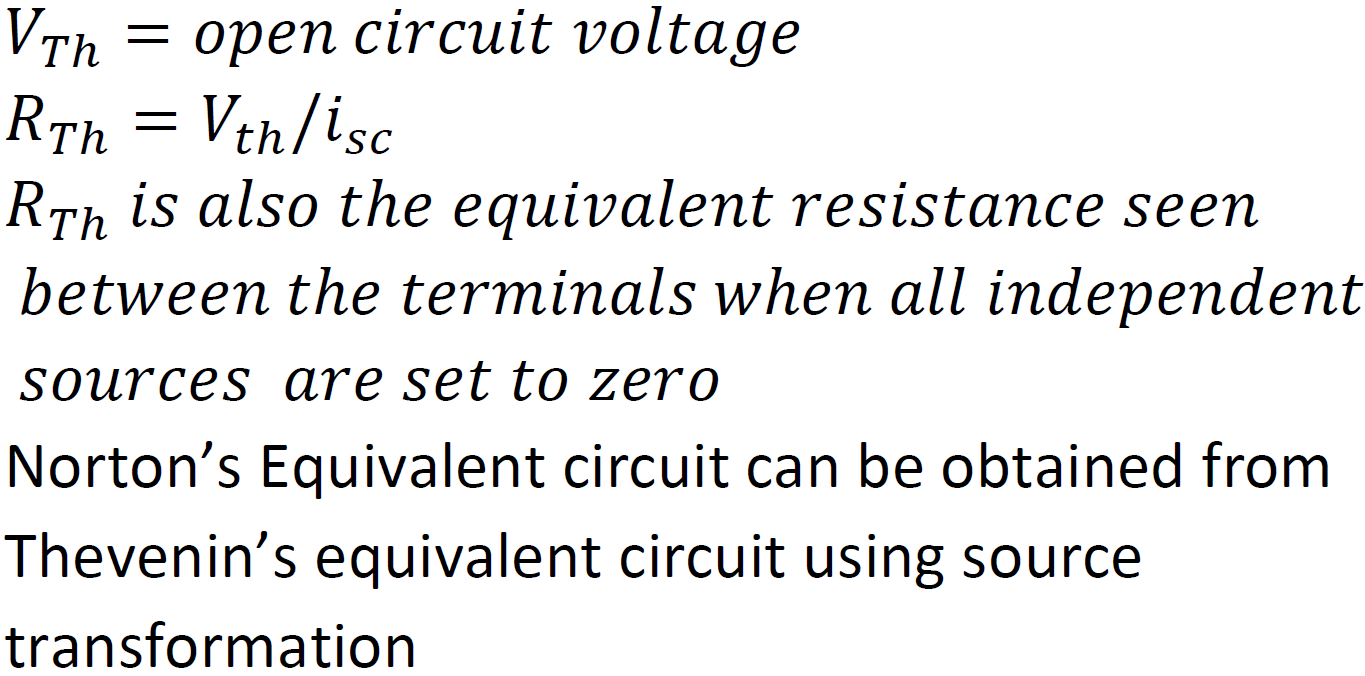
\includegraphics[width=0.2\textwidth]{photos/thevenin_circuits_text.png}\\
  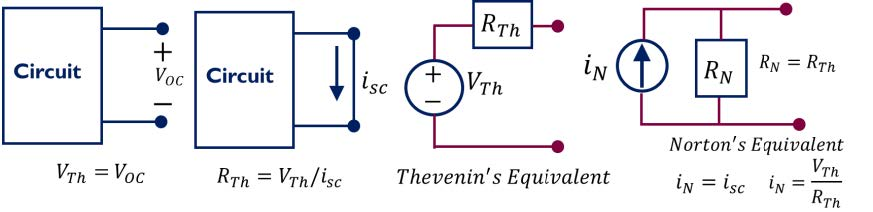
\includegraphics[width=0.2\textwidth]{photos/Thevenins_Equivelent_Circuits.jpg}

  \section*{Voltage and Current Decision}
  \textbf{Voltage Division:}
  \[
    v_x = v_s \frac{R_x}{R_1 + R_2 + \cdots + R_n}
  \]
  Distributes voltage across resistors in series proportionally to their resistance.

  \textbf{Current Division:}
  \[
    i_x = i_s \frac{R_{eq}}{R_x}
  \]
  where \( R_{eq} = R_1 \parallel R_2 \parallel \cdots \parallel R_n \).

  \textbf{Current through a branch:}
  \[
    i_x = i_s \frac{R_{total}}{R_x + R_{total}}
  \]
  If resistances are combined in parallel and a current source is applied.
  These principles aid in determining how voltage or current is shared across circuit components.
  \section*{Capacitor and Inductor}
  %   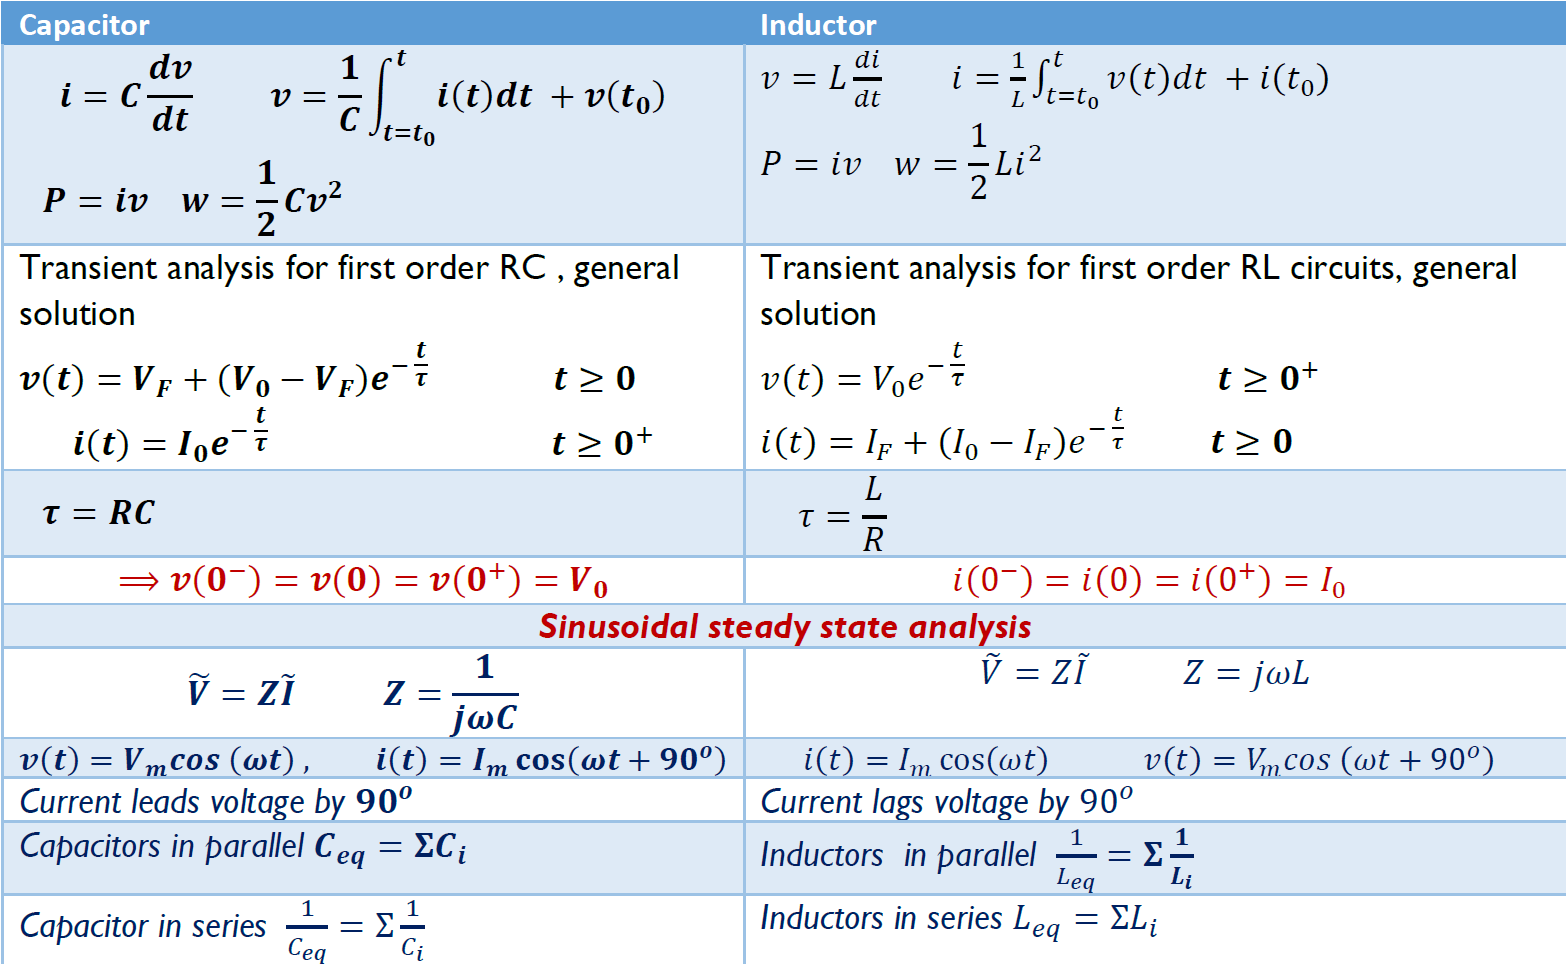
\includegraphics[width=0.2\textwidth]{photos/capacitor_and_inductor.png}
  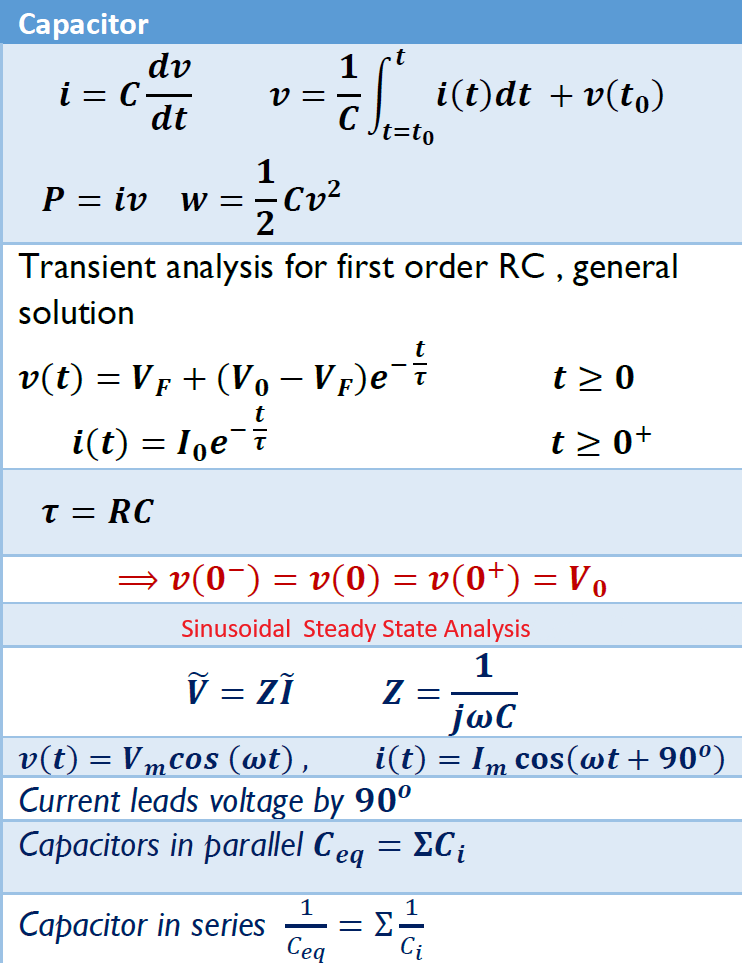
\includegraphics[width=0.2\textwidth]{photos/capacitor.png}\\
  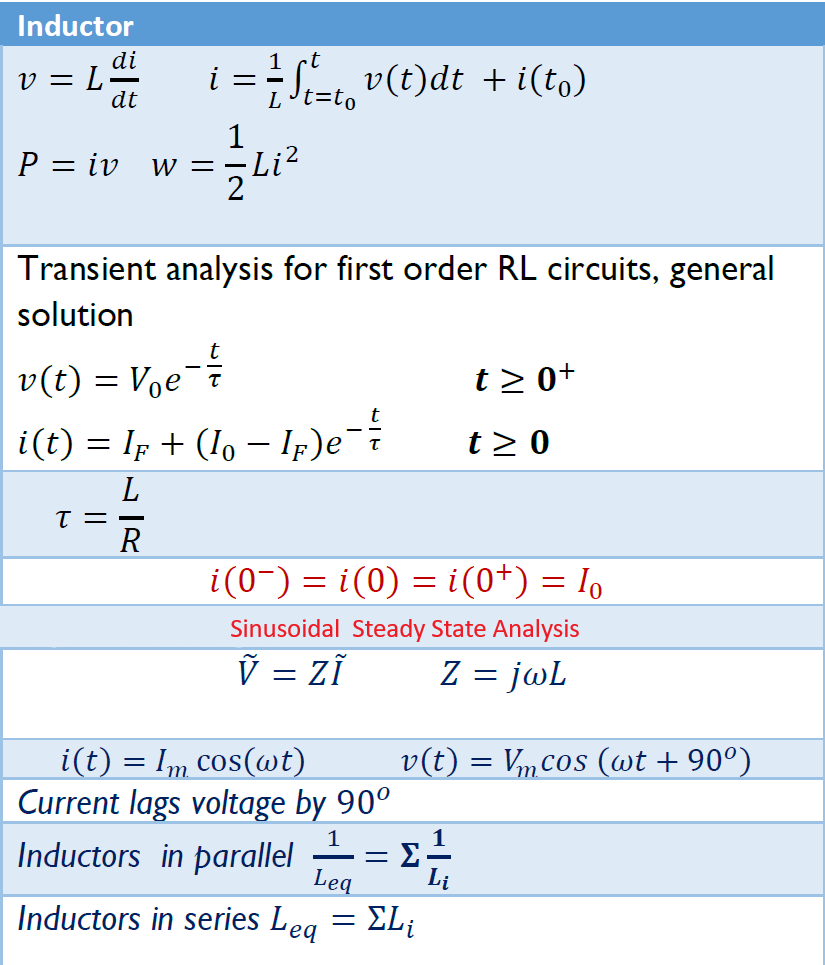
\includegraphics[width=0.2\textwidth]{photos/inductor.png}

  \section*{Phasor Transform}
  \[
    v(t) = V_m \cos(\omega t + \theta_v) \rightarrow \tilde{V} = V_m \angle \theta_v = V_m e^{j\theta_v}
  \]

  \section*{Source Transformation}
  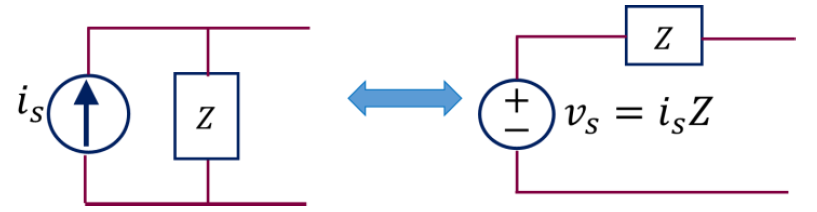
\includegraphics[width=0.2\textwidth]{photos/source_transform.png}

  \section*{Sampling and Quantization}

  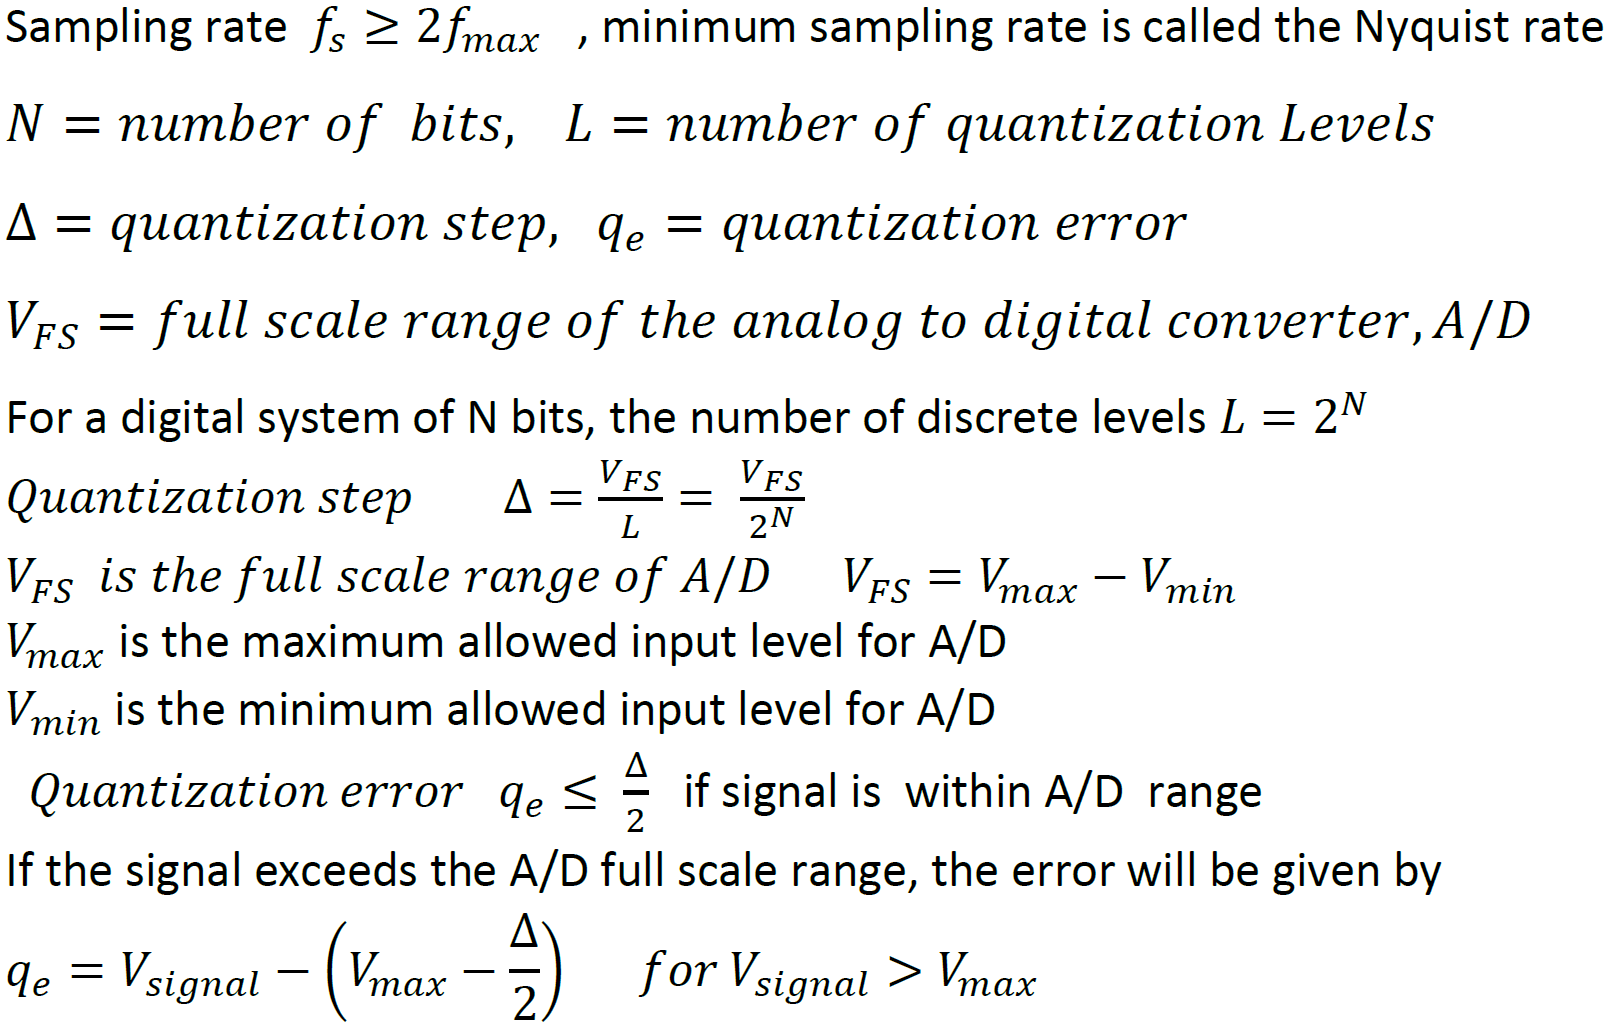
\includegraphics[width=0.2\textwidth]{photos/sampling1.png}\\
  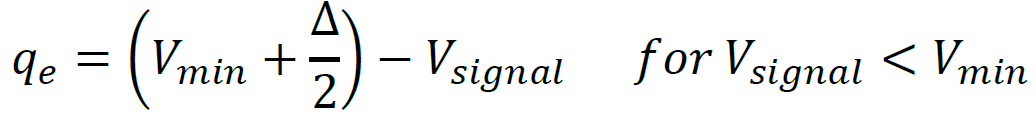
\includegraphics[width=0.2\textwidth]{photos/sampling2.png}
  
%   \textbf{Nyquist Sampling Theorem:}
%   \[
%     f_s \geq 2f_{max}
%   \]
%   The sampling frequency (\(f_s\)) must be at least twice the maximum frequency (\(f_{max}\)) of the signal to avoid aliasing.

%   \textbf{Quantization Levels:}
%   - Number of quantization levels:
%   \[
%     L = 2^N
%   \]
%   where \(N\) is the number of bits in the analog-to-digital converter (ADC).

%   \textbf{Quantization Step Size:}
%   \[
%     \Delta = \frac{V_{FS}}{L} = \frac{V_{FS}}{2^N}
%   \]
%   where \(V_{FS}\) is the full-scale range of the ADC.

%   \textbf{Quantization Error:}
%   - Maximum quantization error:
%   \[
%     q_e \leq \frac{\Delta}{2}
%   \]
%   The error is bounded if the signal is within the ADC range.

%   \textbf{Full-Scale Range:}
%   \[
%     V_{FS} = V_{max} - V_{min}
%   \]
%   \(V_{max}\) and \(V_{min}\) are the maximum and minimum allowed input levels for the ADC.

%   \textbf{Key Definitions:}
%   - \textbf{Aliasing:} If \(f_s < 2f_{max}\), higher frequencies appear as lower frequencies in the sampled signal.
%   - \textbf{Quantization Noise:} The error introduced when mapping a continuous signal to discrete levels.

%   \textbf{Example ADC Calculation:}
%   - For a digital system with 8 bits (\(N = 8\)) and a full-scale range (\(V_{FS}\)) of \(10\text{V}\):
%   \[
%     L = 2^8 = 256, \quad \Delta = \frac{10}{256} = 0.039 \text{V}, \quad q_e \leq 0.0195 \text{V}
%   \]

%   \textbf{Oversampling:}
%   - Using a sampling rate much higher than \(2f_{max}\) improves resolution and reduces quantization noise.

%   \textbf{Reconstruction:}
%   - Original signal can be reconstructed using a low-pass filter if \(f_s \geq 2f_{max}\).

  \section*{Ideal Op-Amps}
  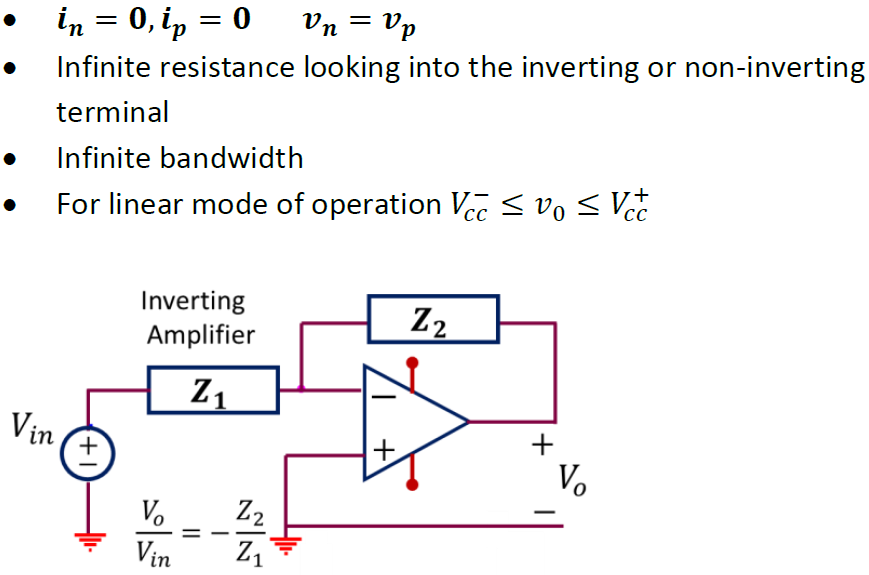
\includegraphics[width=0.2\textwidth]{photos/ideal_opamp1.png}\\
  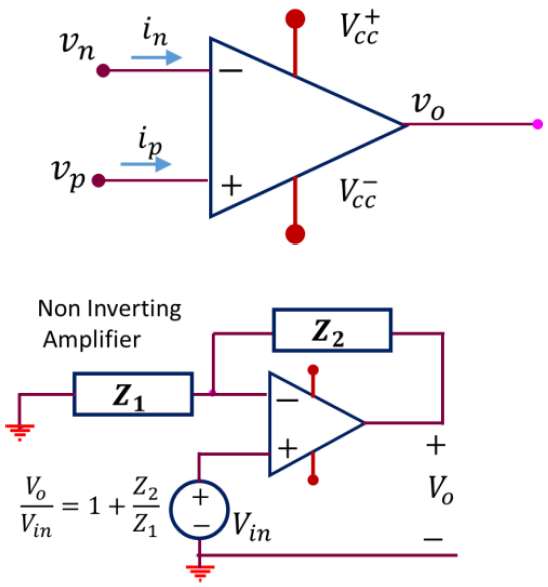
\includegraphics[width=0.2\textwidth]{photos/ideal_opamp2.png}


  \section*{Transfer Functions and the frequency response of linear systems}
  \[
  H(j\omega) = \frac{V_o}{V_{in}}
  \]
  
  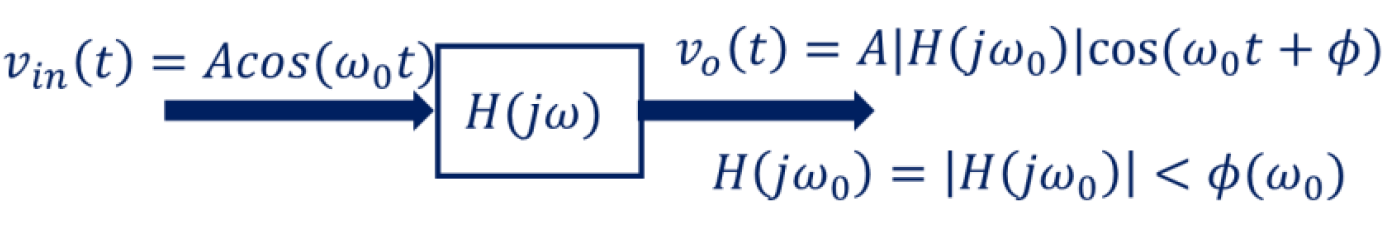
\includegraphics[width=0.2\textwidth]{photos/transfer_func1.png}
\end{multicols*}
\end{document}
